\documentclass[10pt,svgnames,usenames,table]{beamer} %,handout si version papier
\NeedsTeXFormat{LaTeX2e}

\usetheme[compress]{Singapore} % theme

\usepackage[frenchb]{babel}
\usepackage[T1]{fontenc}
\usepackage[utf8x]{inputenc}
\usepackage{lmodern}
\usepackage{amsmath,amsthm,amssymb}        % un packages mathématiques
\usepackage{xcolor}         % pour définir plus de couleurs
\usepackage{graphicx}       % pour insérer des figures
\graphicspath{{../Images/}}
\usepackage{lmodern}
\usepackage{lastpage}
\usepackage{endnotes}
\usepackage{hyperref}

\usepackage{todonotes}


\usepackage{listings}
\usepackage{listingsutf8}

\usepackage{siunitx}
\usepackage{wrapfig}
\usepackage{pdfpages}
\usepackage{verbatim}

\usepackage{caption}
\usepackage{subcaption}

\usepackage{xparse}% for using parameters at the end block

\NewDocumentEnvironment{myfig}{mm}
{\begin{figure}\centering}
{\caption{#2}\label{fig:#1}\end{figure}}

\NewDocumentEnvironment{myfigsub}{mmm}
{\begin{subfigure}[b]{#3\textwidth}}
{\caption{#2}\label{fig:#1}\end{subfigure}}

\newcommand{\mysubfig}[3]
{\begin{myfigsub}{#1}{#2}{#3}
    \includegraphics[width=\textwidth]{#1.png}
\end{myfigsub}}
\newcommand{\mysubfigg}[4]
{\begin{myfigsub}{#1}{#2}{#3}
    \includegraphics[#4, width=\textwidth]{#1.png}
\end{myfigsub}}


\newcommand{\myfullfig}[3]
{\begin{figure}[!ht]
    \centering
    \includegraphics[width=#3\textwidth]{#1.png}
    \caption{#2}
    \label{fig:#1}
\end{figure}}



\DeclareFontFamily{OT1}{pzc}{}
\DeclareFontShape{OT1}{pzc}{m}{it}{<-> s * [1.10] pzcmi7t}{}
\DeclareMathAlphabet{\mathpzc}{OT1}{pzc}{m}{it}

\DeclareMathOperator{\newdiff}{d} % use \dif instead
\newcommand{\dif}{\newdiff\!}
\newcommand{\fpart}[2]{\frac{\partial #1}{\partial #2}}
\newcommand{\ffpart}[2]{\frac{\partial^2 #1}{\partial #2^2}}
\newcommand{\fdpart}[3]{\frac{\partial^2 #1}{\partial #2\partial #3}}
\newcommand{\fdif}[2]{\frac{\dif #1}{\dif #2}}
\newcommand{\ffdif}[2]{\frac{\dif^2 #1}{\dif #2^2}}
\newcommand{\constant}{\ensuremath{\mathrm{cst}}}
\newcommand{\rha}{\hat{r}^n_{MLE}}
\newcommand{\bigoh}{\mathcal{O}}
\newcommand{\F}{\mathcal{F}}

\DeclareMathOperator{\pois}{Pois}
\DeclareMathOperator{\sinc}{sinc}
\DeclareMathOperator{\var}{Var}
\DeclareMathOperator{\argmax}{argmax}

\usepackage{parskip} % Ajoute de l'espace entre les paragraphes et mets l'indentation to 0
\setlength{\parindent}{15pt} % Remets l'indentation par default

\newcommand{\figref}[1]{figure~\ref{fig:#1}}

%\usepackage[svgnames]{color}
%\definecolor{webdarkblue}{rgb}{0,0,0.4}
%\definecolor{webgreen}{rgb}{0,0.3,0}
%\definecolor{webblue}{rgb}{0,0,0.8}

\setbeamercolor{section in head/foot}{use=structure,bg=structure.fg!25!bg} % "Amélioration du jeu de couleur"
%\useoutertheme[subsection=true]{smoothbars} % Pour avoir un rappel de la subsection
\setbeamerfont{frametitle}{series=\bfseries}
\setbeamertemplate{frametitle}[default][center] % Titre centré et bien placé.


% "Fioriture de style" : qd <x-> dans les item, les autres en gris clair
\beamertemplatetransparentcovered


% Comportement des itemize
\setbeamertemplate{itemize item}[ball]
\setbeamertemplate{itemize subitem}[triangle]
\setbeamertemplate{itemize subsubitem}[circle]

%\renewcommand\sfdefault{cmss} % Polices

% Les block arrondis et ombrés dans la couleur que je veux
\setbeamertemplate{blocks}[rounded][shadow=true]
\definecolor{normalBlockColor}{RGB}{255,255,255}
\definecolor{normalTitleBlockColor}{RGB}{0,0,102}
\definecolor{normalBlockTextColor}{RGB}{0,0,0}
\definecolor{normalBlockTitleTextColor}{RGB}{255,255,255}
\definecolor{exampleBlockColor}{RGB}{202,251,197}
\definecolor{exampleTitleBlockColor}{RGB}{166,241,158}
\definecolor{exampleBlockTextColor}{RGB}{0,0,0}
\definecolor{exampleBlockTitleTextColor}{RGB}{0,120,0}
\definecolor{alertBlockColor}{RGB}{248,218,218}
\definecolor{alertTitleBlockColor}{RGB}{244,108,108}
\definecolor{alertBlockTextColor}{RGB}{0,0,0}
\definecolor{alertBlockTitleTextColor}{RGB}{120,0,0}
\setbeamercolor*{block title}{fg=normalBlockTitleTextColor,bg=normalTitleBlockColor}
\setbeamercolor*{block body}{fg=normalBlockTextColor,bg=normalBlockColor}
\setbeamercolor*{block title alerted}{fg=alertBlockTitleTextColor,bg=alertTitleBlockColor}
\setbeamercolor*{block body alerted}{fg=alertBlockTextColor,bg=alertBlockColor}
\setbeamercolor*{block title example}{fg=exampleBlockTitleTextColor,bg=exampleTitleBlockColor}
\setbeamercolor*{block body example}{fg=exampleBlockTextColor,bg=exampleBlockColor}
\setbeamerfont{block title}{size={}}



%------------ fin style beamer -------------------

% Faire apparaître un sommaire avant chaque section
% \AtBeginSection[]{
%   \begin{frame}
%   \frametitle{Plan}
%   \medskip
%   %%% affiche en début de chaque section, les noms de sections et
%   %%% noms de sous-sections de la section en cours.
%   \small \tableofcontents[currentsection, hideothersubsections]
%   \end{frame}
% }


% Pour personnaliser la barre de navigation du dessous
\setbeamertemplate{navigation symbols}{
	%\insertslidenavigationsymbol
	%\insertframenavigationsymbol
	%\insertsubsectionnavigationsymbol
	\quad\textbf{\insertframenumber/\inserttotalframenumber} % Numéro de page
	%\insertsectionnavigationsymbol
	%\insertdocnavigationsymbol
	%\insertbackfindforwardnavigationsymbol
}
% Supprimer les icones de navigation (pour les transparents)
%\setbeamertemplate{navigation symbols}{}

% Mettre les icones de navigation en mode vertical (pour projection)
% \setbeamertemplate{navigation symbols}[vertical]

%\newenvironment{itemize2}%
%	{ \begin{list}%
%		{$\bullet$}%
%		{\setlength{\labelwidth}{30pt}%
%		 \setlength{\leftmargin}{35pt}%
%		 \setlength{\itemsep}{\parsep}}}%
%	{ \end{list} }

%\def\siecle#1{\textsc{\romannumeral #1}\textsuperscript{e}~siècle} % => le \siecle{19}

%\definecolor{codeBlue}{rgb}{0,0,1}
%\definecolor{webred}{rgb}{0.5,0,0}
%\definecolor{codeGreen}{rgb}{0,0.5,0}
%\definecolor{codeGrey}{rgb}{0.6,0.6,0.6}
%\definecolor{webdarkblue}{rgb}{0,0,0.4}
%\definecolor{webgreen}{rgb}{0,0.3,0}
%\definecolor{webblue}{rgb}{0,0,0.8}
%\definecolor{orange}{rgb}{0.7,0.1,0.1}
%\lstset{
%      language=TeX,
%      flexiblecolumns=true,
%      numbers=left,
%      stepnumber=1,
%      numberstyle=\ttfamily\tiny,
%      keywordstyle=\ttfamily\textcolor{blue},
%      stringstyle=\ttfamily\textcolor{red},
%      commentstyle=\ttfamily\textcolor{codeGreen},
%      breaklines=true,
%      extendedchars=true,
%      basicstyle=\ttfamily\scriptsize,
%      showstringspaces=false,
%      morekeywords={usepackage,documentclass,begin,textbf,textit,texttt,ref,includegraphics,caption,label,setlength,mathbb,notag,frac,num,si,ang,SI,textwidth,percent,meter,ohm,joule,second,more,section,subsection,tableofcontents,setstretch,TeX,LaTeX,huge,sffamily,emph,chemfig,pageref,vpageref},
%      frame=single,
%      extendedchars=true,
%      inputencoding=utf8x
%    }
%\lstset{inputencoding=utf8/latin1}

\renewcommand{\subsection}[1]{}

\usepackage{empheq}
\usepackage{amsmath}
\definecolor{gris}{RGB}{228,228,228}
\definecolor{bleu}{RGB}{34,148,255}
\definecolor{darkgray}{rgb}{0.3,0.3,0.3}


\institute{LFSAB1507}
\title{\textbf{Picture deblurring}\\Project of applied mathematics }
\author{Jonathan \textsc{Berthe} \and Arnaud \textsc{Cerckel} \and Benoît \textsc{Legat} \and Geoffroy \textsc{Vanderrreydt}}

\date{}

\usepackage{caption}
\usepackage{subcaption}

 
\begin{document}


\begin{frame}
\maketitle
\vspace{-30pt}
\begin{figure}[h!]
\centering
\begin{subfigure}{0.4\textwidth}
\includegraphics[width= \textwidth]{../Images/Results/reel/foot/Original.jpg}
\end{subfigure}
~
\begin{subfigure}{0.4\textwidth}
\includegraphics[{width= \textwidth}]{../Images/Results/reel/foot/L.png}
\end{subfigure}
\end{figure}
\end{frame}

\AtBeginSection[]
  {
     \begin{frame}<beamer>
     %\frametitle{\insertsection}
     \tableofcontents[hideothersubsections]
     \end{frame}
  }

  
\chapter{Introduction}

Nowadays, more and more people deal with pictures, especially when they want to immortalize a special moment with their smartphone. But the pictures are often blurred because of a motion of the camera, the motion of a subject or a misfocus of the camera or for any other reason. That's why processing images, and especially deblurring, has become an important aspect in people's daily lives.

This report contains a study about the blur effect on an image and proposes some algorithms to remove that effect as much as possible. Blur can occur for many reasons. It is impossible to have a general method that solves all types of blur effects. That is why we only focus on two typical situations. In the first one, the picture has been taken from a moving train travelling with a known or unknown speed. In the second chosen situation, a security camera takes a picture with a moving subject. We dispose of several statistical images without any moving subject and we deblur the part of the image where we detected the moving subject.

The report begins with a clear and precise definition of what actually an image is and it gives a mathematical formulation for the blur problem. A good mathematical model of the blur effect is a key step in the understanding of this phenomena. Then extracting some information of the specified situation helps to get a more accurate model.

The mathematical modelisation is followed by the general strategy that we will follow to solve a deblurring problem. In this chapter, you will encounter our special item that we wanted to focus on: fast computing. Even if the main goal of this report is to achieve good results of deblurring, we also treated the case where the quickiness is more important than the quality. This especially applies on the situation with the security camera. For example, a security man observes the images of a camera in a room on his screen. He only needs an idea of what is going on in the room but right now, on this moment and not 1 hour ago.

Subsequently, we go in a deeper analysis of what is described in the general strategy. We explain the methods we use to deblur and compare them for different images and different types of blur.

Finally, we end with the strengths and the weaknesses of this project and some suggested improvements. A conclusion resumes the main point of this report. All the algorithms have been implemented with \texttt{Matlab} and the codes have been included in the appendices.

\section[Math. Formulat.]{Mathematical formulation}

\begin{frame}
	\frametitle{Mathematical Model}
	Continuous Model
	\begin{itemize}
	\item What is an image? $f:\Omega \rightarrow \mathbb{R}: (x,y) \mapsto f(x,y)$
	\item What is blurring? $g(x,y) = f(x,y) \ast h(x,y) + e(x,y)$
	\end{itemize}
	Discrete Model
	\begin{itemize}
	\item What is an image? $f(m,n)$ for $m=1...M$, $n=1...N$
	\item What is blurring? $G = HF + E$, $G,F,E \in \mathbb{R}^{M \cross N}$, $H \in \mathbb{R}^{M \cross M}$
	linear system: $\mathpzc{g} = \tilde{H}\mathpzc{f} + \mathpzc{e}$, where $\mathpzc{f} = vec(F)$ and $\tilde{H} = I_n \otimes H$
	\end{itemize}
\end{frame}

\section[G. Strategy]{General Strategy}

\begin{frame}
	\frametitle{General Strategy}
	\begin{enumerate}
	\item Estimation of PSF
		\begin{enumerate}
		\item angle: Radon transform or Gabor filter
		\item length: cepstrum
		\end{enumerate}
	\item Deconvolution with estimated PSF. 3 methods:
		\begin{enumerate}
		\item Lucy-Richardson
		\item Wiener
		\item Regularization
		\end{enumerate}
	\end{enumerate}
	
	\begin{description}
	\item[train case] directly applied
	\item[camera case] first detect foreground and apply only on this part of the image
	\end{description}
\end{frame}
\section{Estimation of the PSF}
\subsection{angle estimation with the Gabor filter}

The Gabor filter is a gaussian filter modulated by a sinusoidal wave. The function of this filter is given by:
\begin{equation}
B(x,y)=dfrac{1}{2\pi \sigma_x \sigma_y} exp\left[-\frac{1}{2}\left(\frac{x^2}{\sigma_x^2}+ \frac{y^2}{\sigma_y^2} \right) -j\omega(xcos\phi + ycos\phi)\right],
\label{filtreGabor}
\end{equation}
where $\sigma_x$ and $\sigma_y$ are the standard deviations in the $x$ and $y$ directions. The parameters $\phi$ and $\omega$ are the direction and the frequency of the filter respectively. Only $\phi$ will vary while the other parameters stay fixed. According to the article \cite{dash2014motion}, experimentation has shown that good values for $\sigma$ and $\omega$ are $3$ and $1.75$ respectively. The method consists in applying the Gabor filter to the power spectrum of the blurred image and then detecting the blur angle $\alpha_{blur}$ by searching for the $\phi$ that gives the highest response value. This value can be calculated using $L_2$ norm. The $\phi$ obtained by this method is the blur angle. Here are the steps of the algorithm:

1. computation of the spectrum of the blurred image by a two dimensional Fourier transform\\
2. taking the logarithm of it\\
3. convolving this with the Gabor function given by equation $(\ref{filtreGabor})$ for different $\phi$, the result is $R(\phi)$\\
4. for every $\phi$, taking the $L_2$ norm: $||R(\phi)||_2$
5. the blur angle is the parameter $phi$ that gives the biggest norm:
\begin{equation}
\alpha_{blur} = arg \left\lbrace max_{\phi}R(\phi)\right\rbrace.
\end{equation}

This algorithm is implemented by our matlab function $angle_estimator_Gabor(f,thetamin, thetamax)$, where the input $f$ is the blurred image. The parameter $\phi$ will vary from $thetamin$ to $thetamax$. If those inputs are not specified, we set them to $0$ for $thetamin$ and $180$ for $thetamax$.

All the tests we have done with this method didn't give satisfactory results. We implemented the method exactly as we just described but we couldn't find any error that leads to those bad results. 

%We made some tests with the picture of the little girl on figure (??). We blurred that image everytime with 
%$meth=2$ in our matlab function $blur$. The length was fixed at $20$ and the tests were made for different angles. The results are given in figure

\begin{figure}
\centering
\includegraphics[scale=0.7]{}
\end{figure}



\section{Inverse filter}
The first and most obvious type of deconvolution is using an inverse filter. We have a blurred image $g$, we found an estimation of the psf ($h_e$) in the previous section %TODO ça sera tjs des sections ?
. So we are theoretically ready to find the original image. We had
\begin{equation}
 g =  h*f,
\end{equation}
in frequency domain
\begin{equation}
G = HF. 
\end{equation}

Using $H_e$, the estimated psf in frequency domain, we can get $F_e$ an so $f_e$ by 
\begin{equation}
F_{e} = H_{e}^{-1} G
\end{equation} 

However it's clear that if we add some noise this model doesn't work anymore. Indeed as shown on figure \ref{fig:psfFFT}, $H_e$ has some value near zero. So when we divide $G$ by this, the noise is strongly amplified by the value near zero. This problem explains the results obtained on figure XXX. %TODO  

\begin{figure}
\centering
\includegraphics[scale=0.5]{../Images/psfFFT.png}
\caption{FFT of the psf}
\label{fig:psfFFT}
\end{figure}



\section{Lucy Deconvolution}



\section{Wiener Deconvolution}
 Another deconvolution is the wiener one. 




\section{Regularisation}
%TODO
The last deconvolution method is the deconvolution using regularized filter. 
Instead of a simple inverse 
\begin{equation}
\sum_{m,n} \left[ (g(m,n) - h(m,n)*f(m,n))^2 + \alpha (l(m,n)*f(m,n))^2 \right]
\end{equation}

\begin{equation}
\sum_{k,l} \{ [G(k,l) - H(k,l)F(k,l)]^2 + \alpha [L(k,l)F(k,l)]^2\}
\end{equation}


\begin{equation}
\hat{F}(k,l) = \frac{H(k,l)}{|H(k,l)|^2 + \alpha |L(k,l)|^2} G(k,l)
\end{equation}
\section{Complementary Treatment}

\subsection{Estimation of the noise-to-signal power ratio (NSR)}
\label{subsec:NSREstimation}
Deconvolution by the method of Wiener needs the NSR of the additive noise in the image. The problem of computing the NSR is that we need the original image, which we usually don't have, otherwise deblurring would have no meaning anymore. That is why we try to estimate the SNR by the following reasoning. The pixels of a zone that represent a background (e.g. an area of a blue sky) should be approximatively constant. So the variance of this area would me mostly due to the noise. So we will estimate the power of noise by the variance of such an area. This is the main idea of our matlab function $nsrEstimation(f,psf)$, with $f$ the processed image. % ca sert à quoi psf? %cmt choisir intervention humaine ou pas? if true..?

This function proposes two ways to handle this. In the first one, the user must select an area that he considers as background. In the second way, the function selects automatically five regions: four in the corners and one in the center. It computes the variance for each region and it takes the zone with the least variance. The second method is probably less precise because the predefined regions might not represent parts of a background. But it has the advantage that it doesn't need a human intervention which means there is less work for the user and deblurring also goes faster. Indeed, it's not possible to ask the user to detect a region of background everytime you want to deblur an image when the goal is to have an algorithm near to real-time.

Once we have an estimation for the noise power, we compute the variance of the whole image to get the signal power and we divide the first value by the scond one, giving an estimation of the NSR.


\subsection{Blur metrics}

To compare different methods of deblurring, we need to be able to give the perceptual quality of an image. Suppose we have the original image $F$ and we want to estimate the quality of another image $\hat{F}$ that is a blurred version of $F$ or an approximation of $F$ after a deblurring operation. An easy way to do this is computing the Mean Square Error (MSE) between both images:
\begin{equation}
MSE=\frac{1}{MN} \sum\limits_{m=1}^{n=1}\left(F(m,n)-\hat{F}(m,n)\right)^2.
\end{equation}

The problem of this method is that it highly depends on the scale of intensity of the image. That's why we prefer the Peak Signal-to-Noise Ratio (PSNR) that avoid this problem:
\begin{equation}
PSNR = -10 log \frac{MSE}{S^2},
\end{equation}
where $S$ is the maximum value that a pixel can reach (255 for 8bits coding). Here the bigger the PSNR is, the better the quality of the image.

The problem of both methods is that we need the original image. That is only possible when we blur the images ourselves and we test our different deblurring methods. But in a real situation, we don't know $F$. The only image we have is the blurred image $G$ and the result of a deblurring method $\hat{F}$, so we can apply MSE and PSNR to those images. But we still only get an estimation of how close both images are, not of the blur intensity itself. Our next method determines the quality of an image objectively and without referential image. The technique that we found is a no-reference blur metric that is based on the analysis of the spread of the edges in an image. No-reference means that the metric is not relative to the original but is a absolute value associated to an image.

When an image is blurred, its high spatial frequency values in the spectrum are attenuated. Blur is perceptually apparent along edges so the technique is based on the smoothing effect of it on the edges. According to SOOOOOURCE (marziliano2002),it is sufficient to measure blur along vertical edgdes. Here is the algorithm:\\
First we detect the edges by a Sobel filter for example. Then we scan each row of the image. When we detect a pixel that corresponds to an edge, we look for the local maximum and minimum on that row. The distance (in pixels) between those extrema represents the local blur. Finally, we get the global blur measure for whole the image by averaging the local blur values over all edge locations.

The matlab function $bordSobel(I,meth,tresh,direction)$ implements this algorithm. The inputs are the processed image $I$, the method used to determine the edges ($1=Sobel, 2=Prewitt, 3=Canny$), a treshold for those methods that is fixed at $0.0215$ if it is not specified and finally the direction of the edges (vertical or horizontal).

%TODO résultats
%TODO changer nom de bordSobel car ca peut une autre meth que Sobel


\subsection{EdgeTaper}

One of the main characteristic of the frequency domain is its periodicity. It means that at the edges of the pictures \todo{To be continued after getting a nap} 

\subsection{RGB - grayscaled images : analysis and treatment}

As described in the mathematical model, gray-scaled images and color images differ in their mathematical structure. The easiest way for Matlab to manage the color space is adopt a RGB (Red-Green-Blue) representation such that the output for a certain point of the map is a 3-dimensional vector (one dimension per primitive color) instead of a scalar in the case of a gray-scaled image. The image is thus represented by a matrix of three dimensions and the final color is a additive synthesis of these three components.
 
In the case of our work, we have adapted the program so that it works for both types of images (RGB or gray-scaled one). It is also possible for a user to choose to convert the image to be processed in gray-scaled with the GUI (which operates the rgb2gray.m function). The advantage of converting an image to gray-scaled before the process is a saving time (one-dimensional processing instead of 3 for RGB). For example, the gain of time by converting the images from the surveillance camera can be quite important. Furthermore, according to intended use, it is not always necessary to have a final color image (ie the deblurring of a registration plate).
\section[Bonus Item]{Bonus Item : ``Real-time''}
\begin{frame}{PSF estimation}

The angle and length estimation are achieved with a $256 \times 256 $ pixels square. 
 
\begin{figure}[h]
\centering
\begin{subfigure}{0.4\textwidth}
\includegraphics[width= \textwidth]{../Images/SagarShortEstimation.png}
\vspace{-20pt}
\caption{ $256\times 256$ centered crop of the picture. }
\label{fig:SagarShort}
\end{subfigure}
~
\begin{subfigure}{0.4\textwidth}
\includegraphics[{width= \textwidth}]{../Images/SagarLongEstimation.png}
\vspace{-20pt}
\caption{The whole image.}
\label{fig:SagarLong}
\end{subfigure}
\caption{Different matrix's size for the PSF estimation.}
\end{figure}
\end{frame}

\begin{frame}{Resizing}
 
Challenge : Artifacts may occur during the resizing process. 

\begin{figure}
\centering
\begin{subfigure}{0.4\textwidth}
\includegraphics[width= \textwidth]{../Images/bricksCompressed.png}
\vspace{-20pt}
\caption{Nearest-Neighbor algorithm. }
\label{fig:bricksCompressed}
\end{subfigure}
~
\begin{subfigure}{0.4\textwidth}
\includegraphics[width = \textwidth]{../Images/bricksLanczos.png}
\vspace{-20pt}
\caption{Lanczos2 algorithm.}
\label{fig:bricksLanczos}
\end{subfigure}
\caption{Picture resized using different algorithms}
\end{figure}

\end{frame}

\section[Camera]{Camera}
\subsection{Background estimation}
\begin{frame}[allowframebreaks]
	\frametitle{Background estimation }
	\begin{enumerate}
	\item Input: $k$ images (size $M$x$N$ for gray-scaled image) from fixed camera
	\item Output: Matrix M (size $M$x$N$). In (m,n), means  of the k images only if ($i = 1,\cdots, k)$:	
	$$I_i (m,n) \in [med(m,n) - Inter(m,n); med(m,n) + Inter(m,n)]$$
    \item Examples
	\end{enumerate}

\begin{figure}[h]
\centering
\begin{subfigure}{0.20\textwidth}
\includegraphics[width= \textwidth]{../Images/Camera/Autoroute/fg/06.jpg}
\end{subfigure}
~
\begin{subfigure}{0.20\textwidth}
\includegraphics[{width= \textwidth}]{../Images/Camera/Autoroute/fg/07.jpg}
\end{subfigure}
~
\begin{subfigure}{0.20\textwidth}
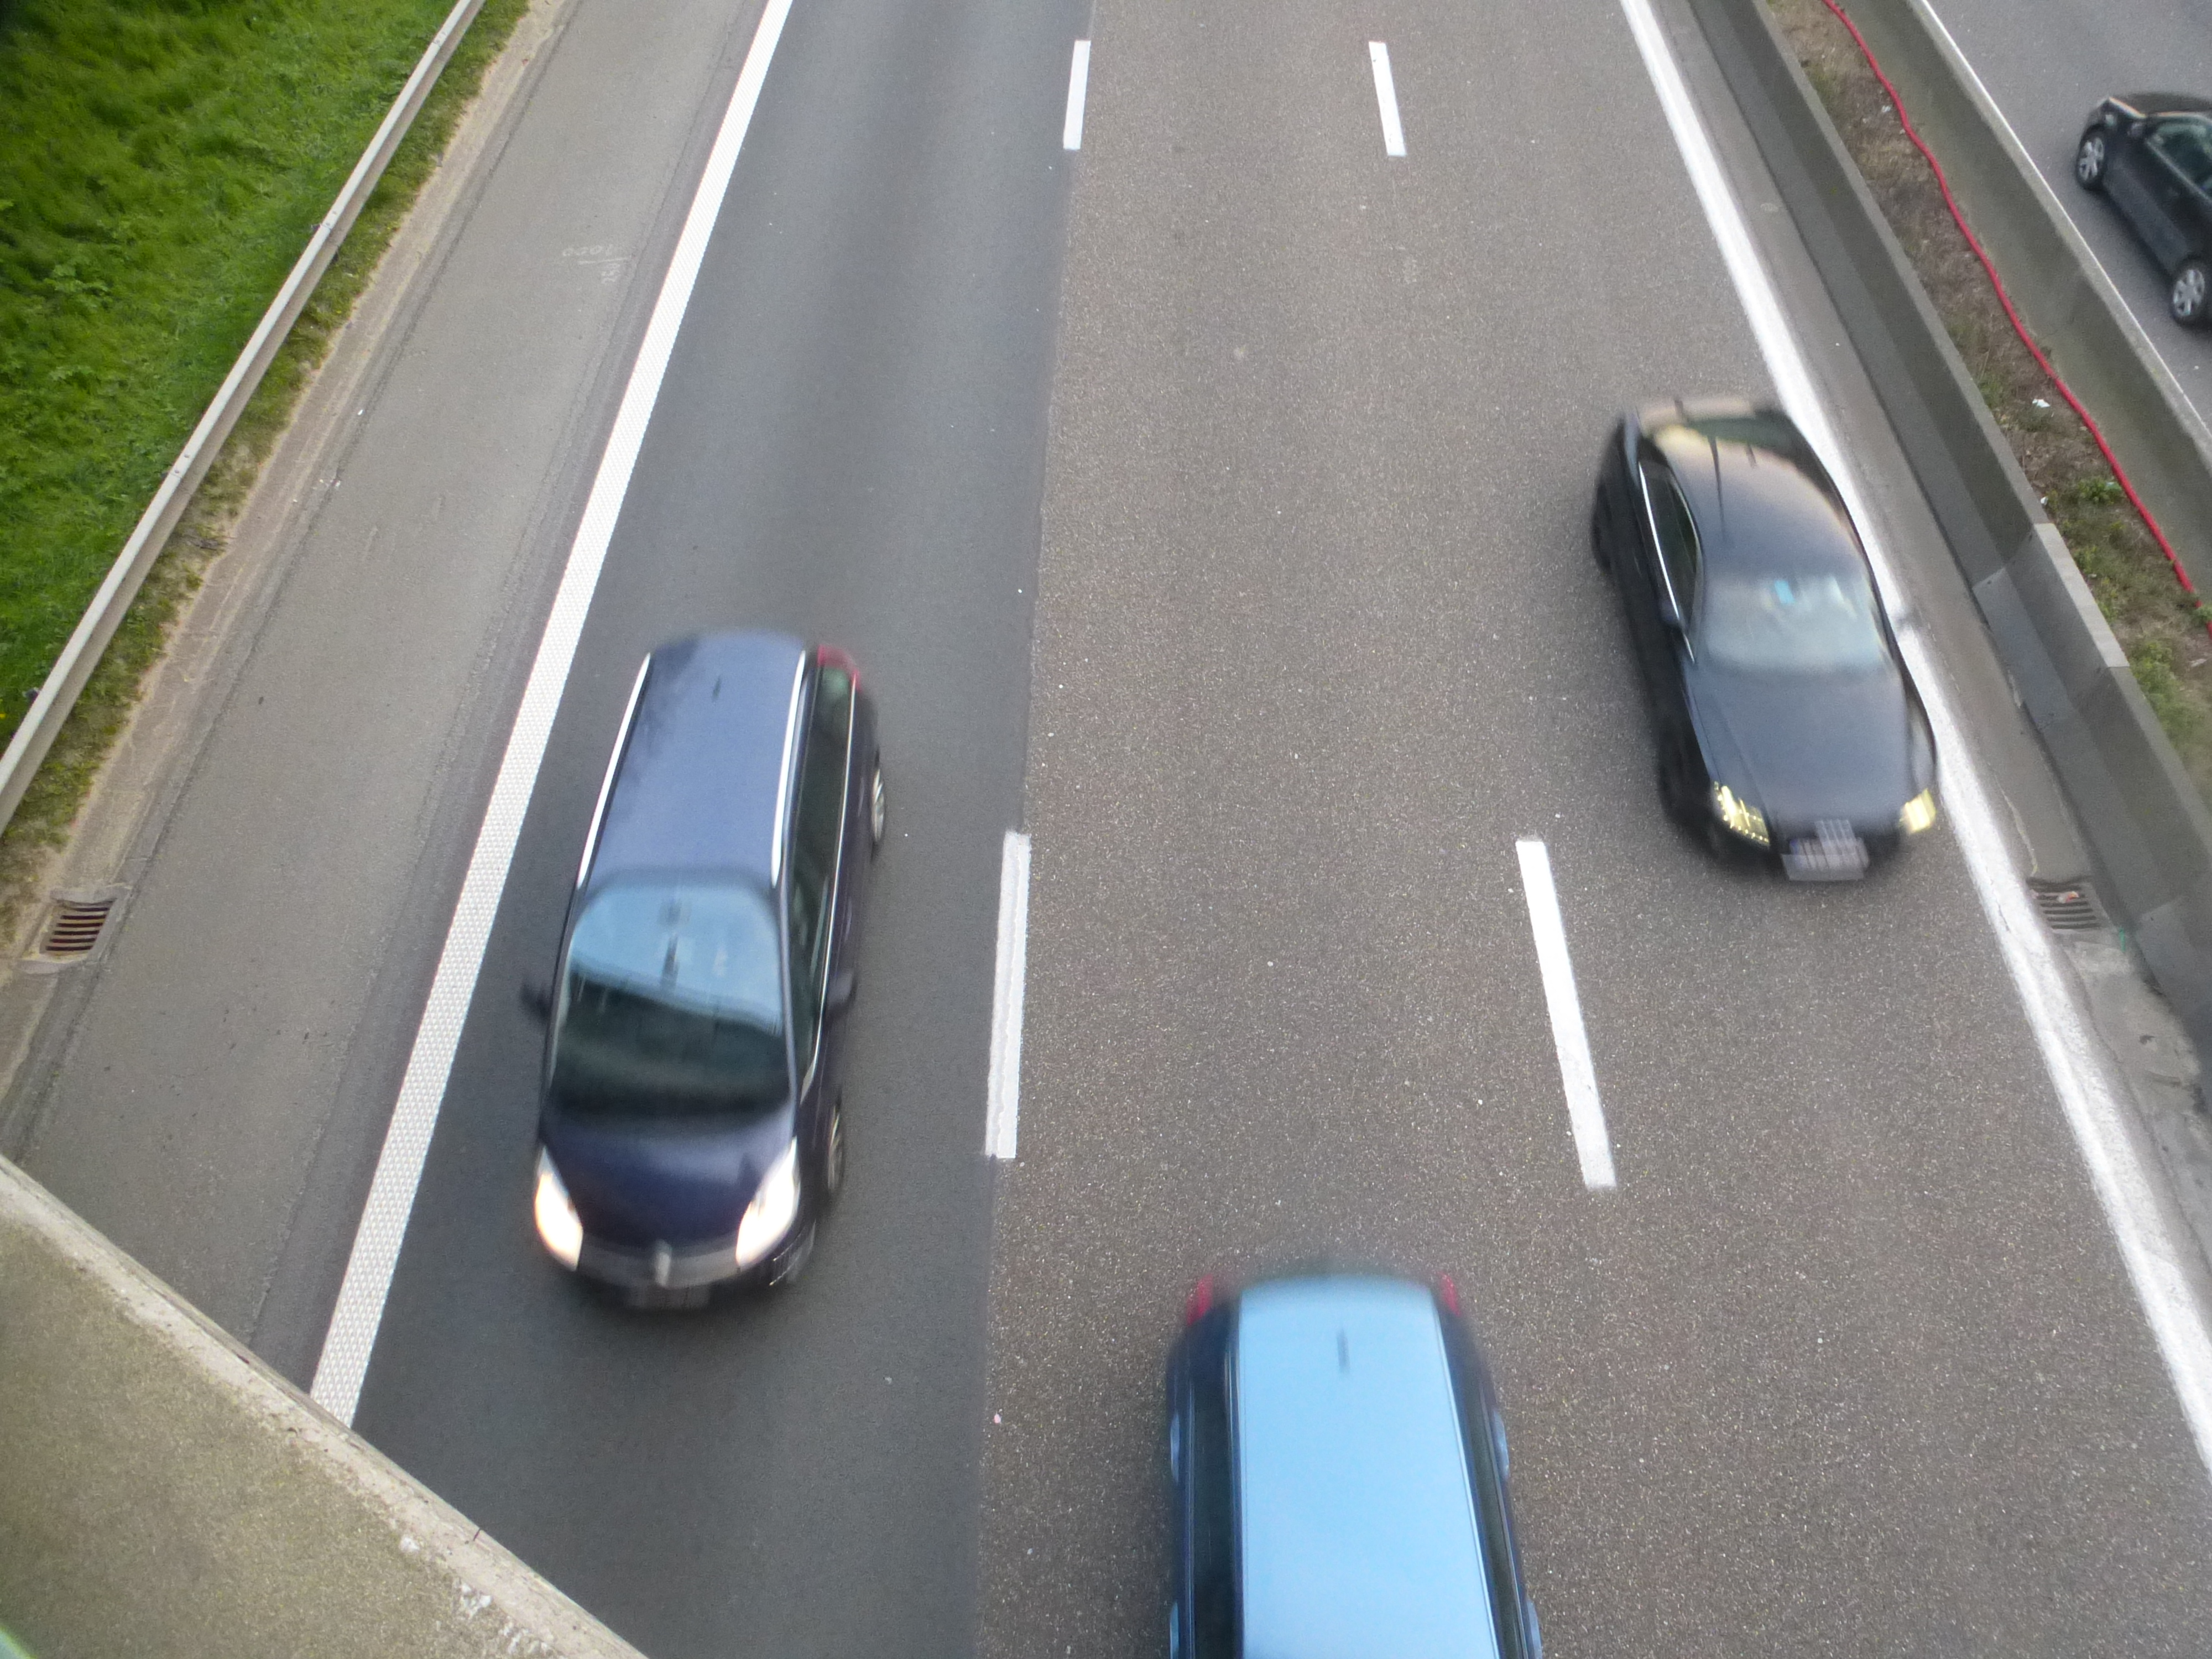
\includegraphics[{width= \textwidth}]{../Images/Camera/Autoroute/fg/13.jpg}
\end{subfigure}
~
\begin{subfigure}{0.20\textwidth}
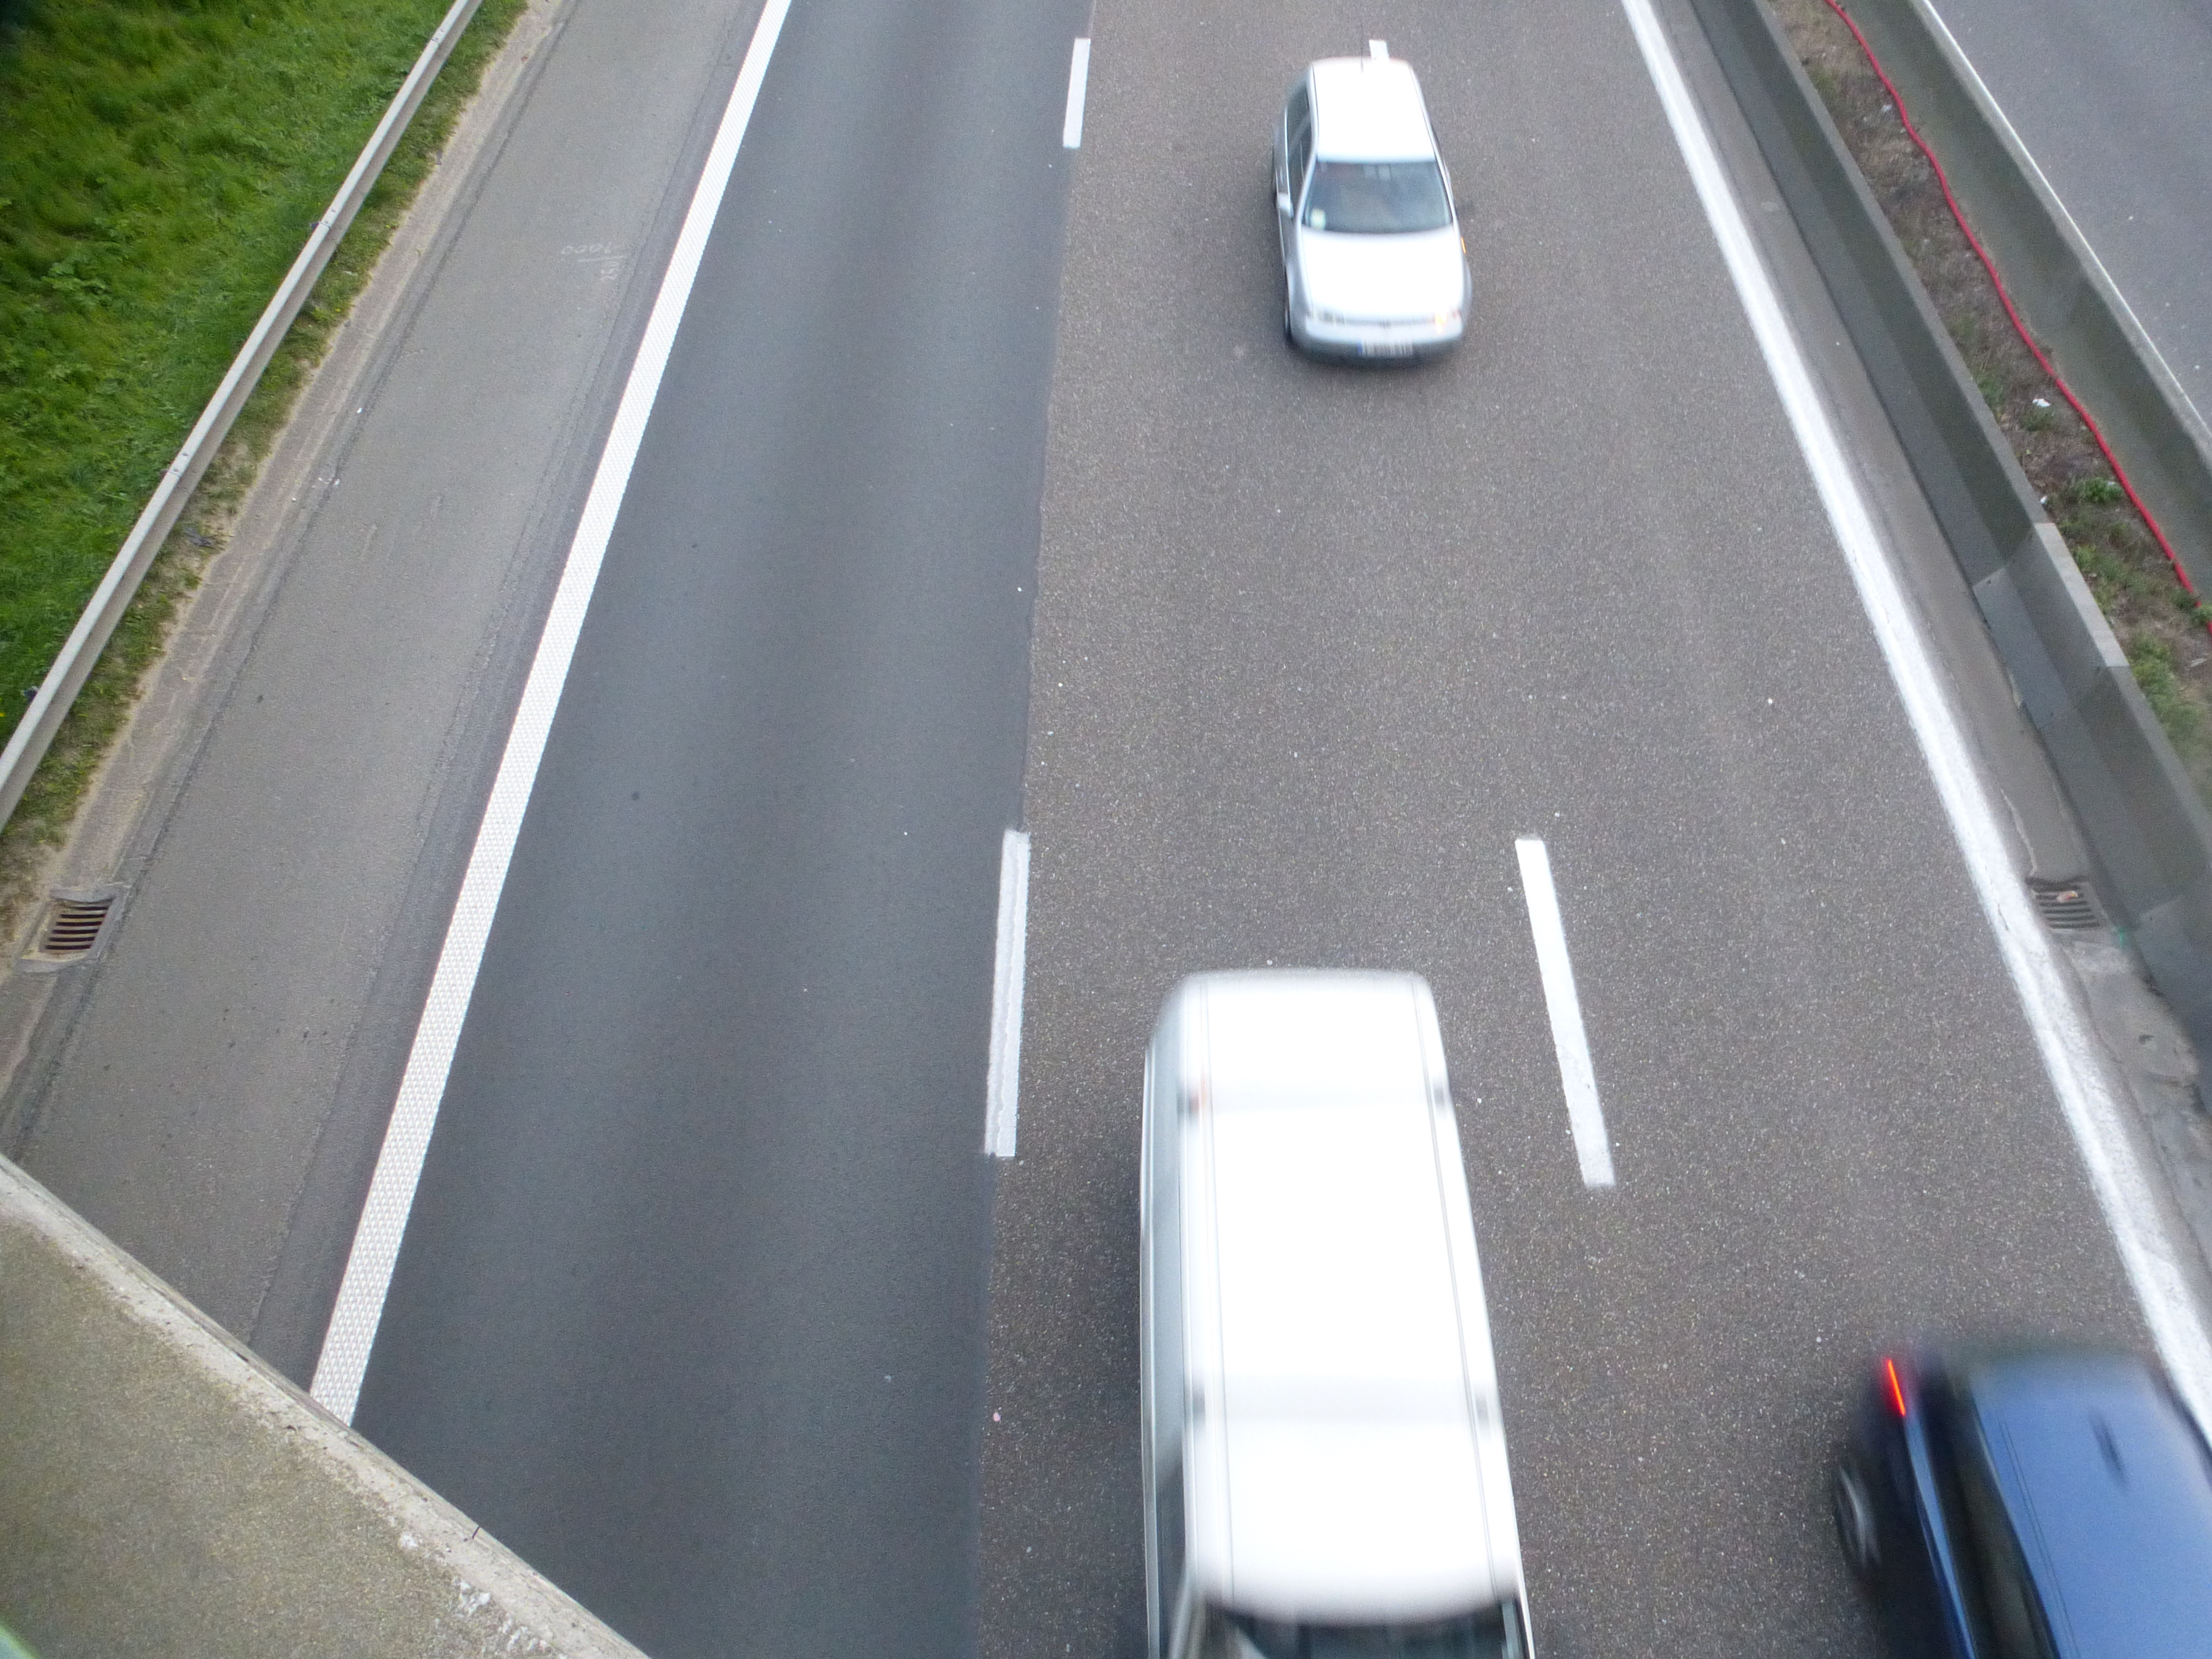
\includegraphics[{width= \textwidth}]{../Images/Camera/Autoroute/fg/14.jpg}
\end{subfigure}
~
\begin{subfigure}{0.20\textwidth}
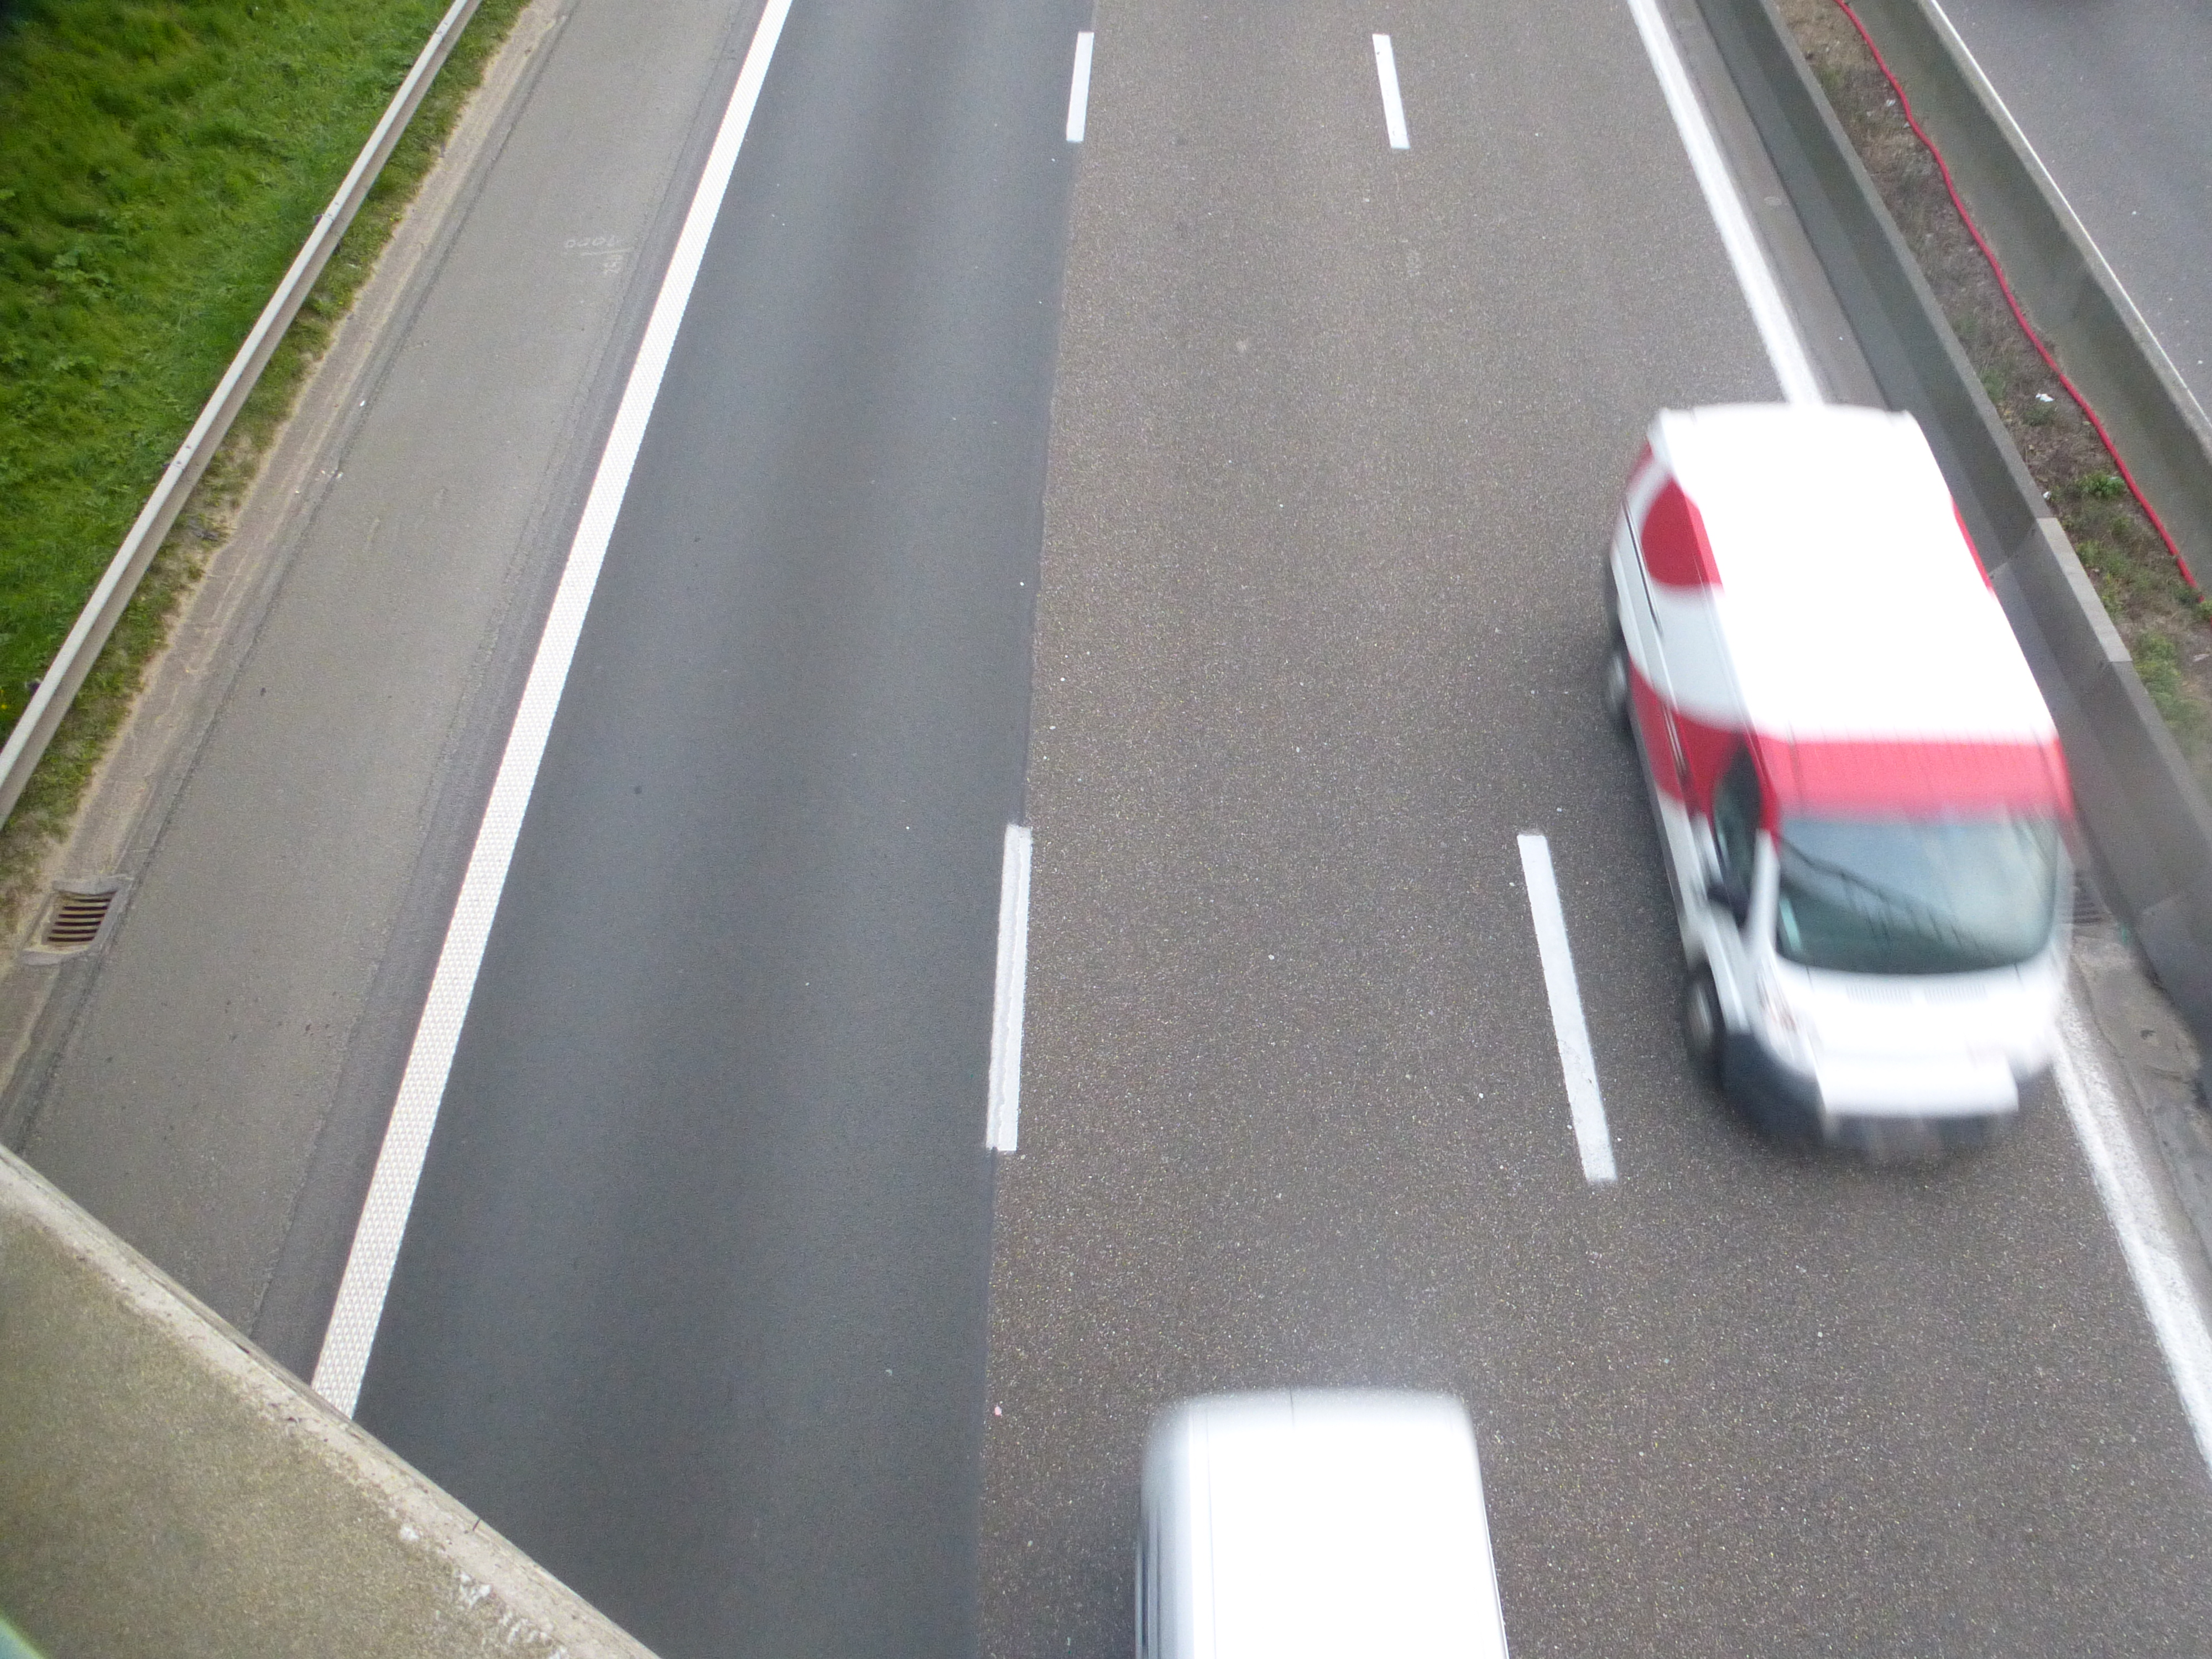
\includegraphics[{width= \textwidth}]{../Images/Camera/Autoroute/fg/15.jpg}
\end{subfigure}
~
\begin{subfigure}{0.20\textwidth}
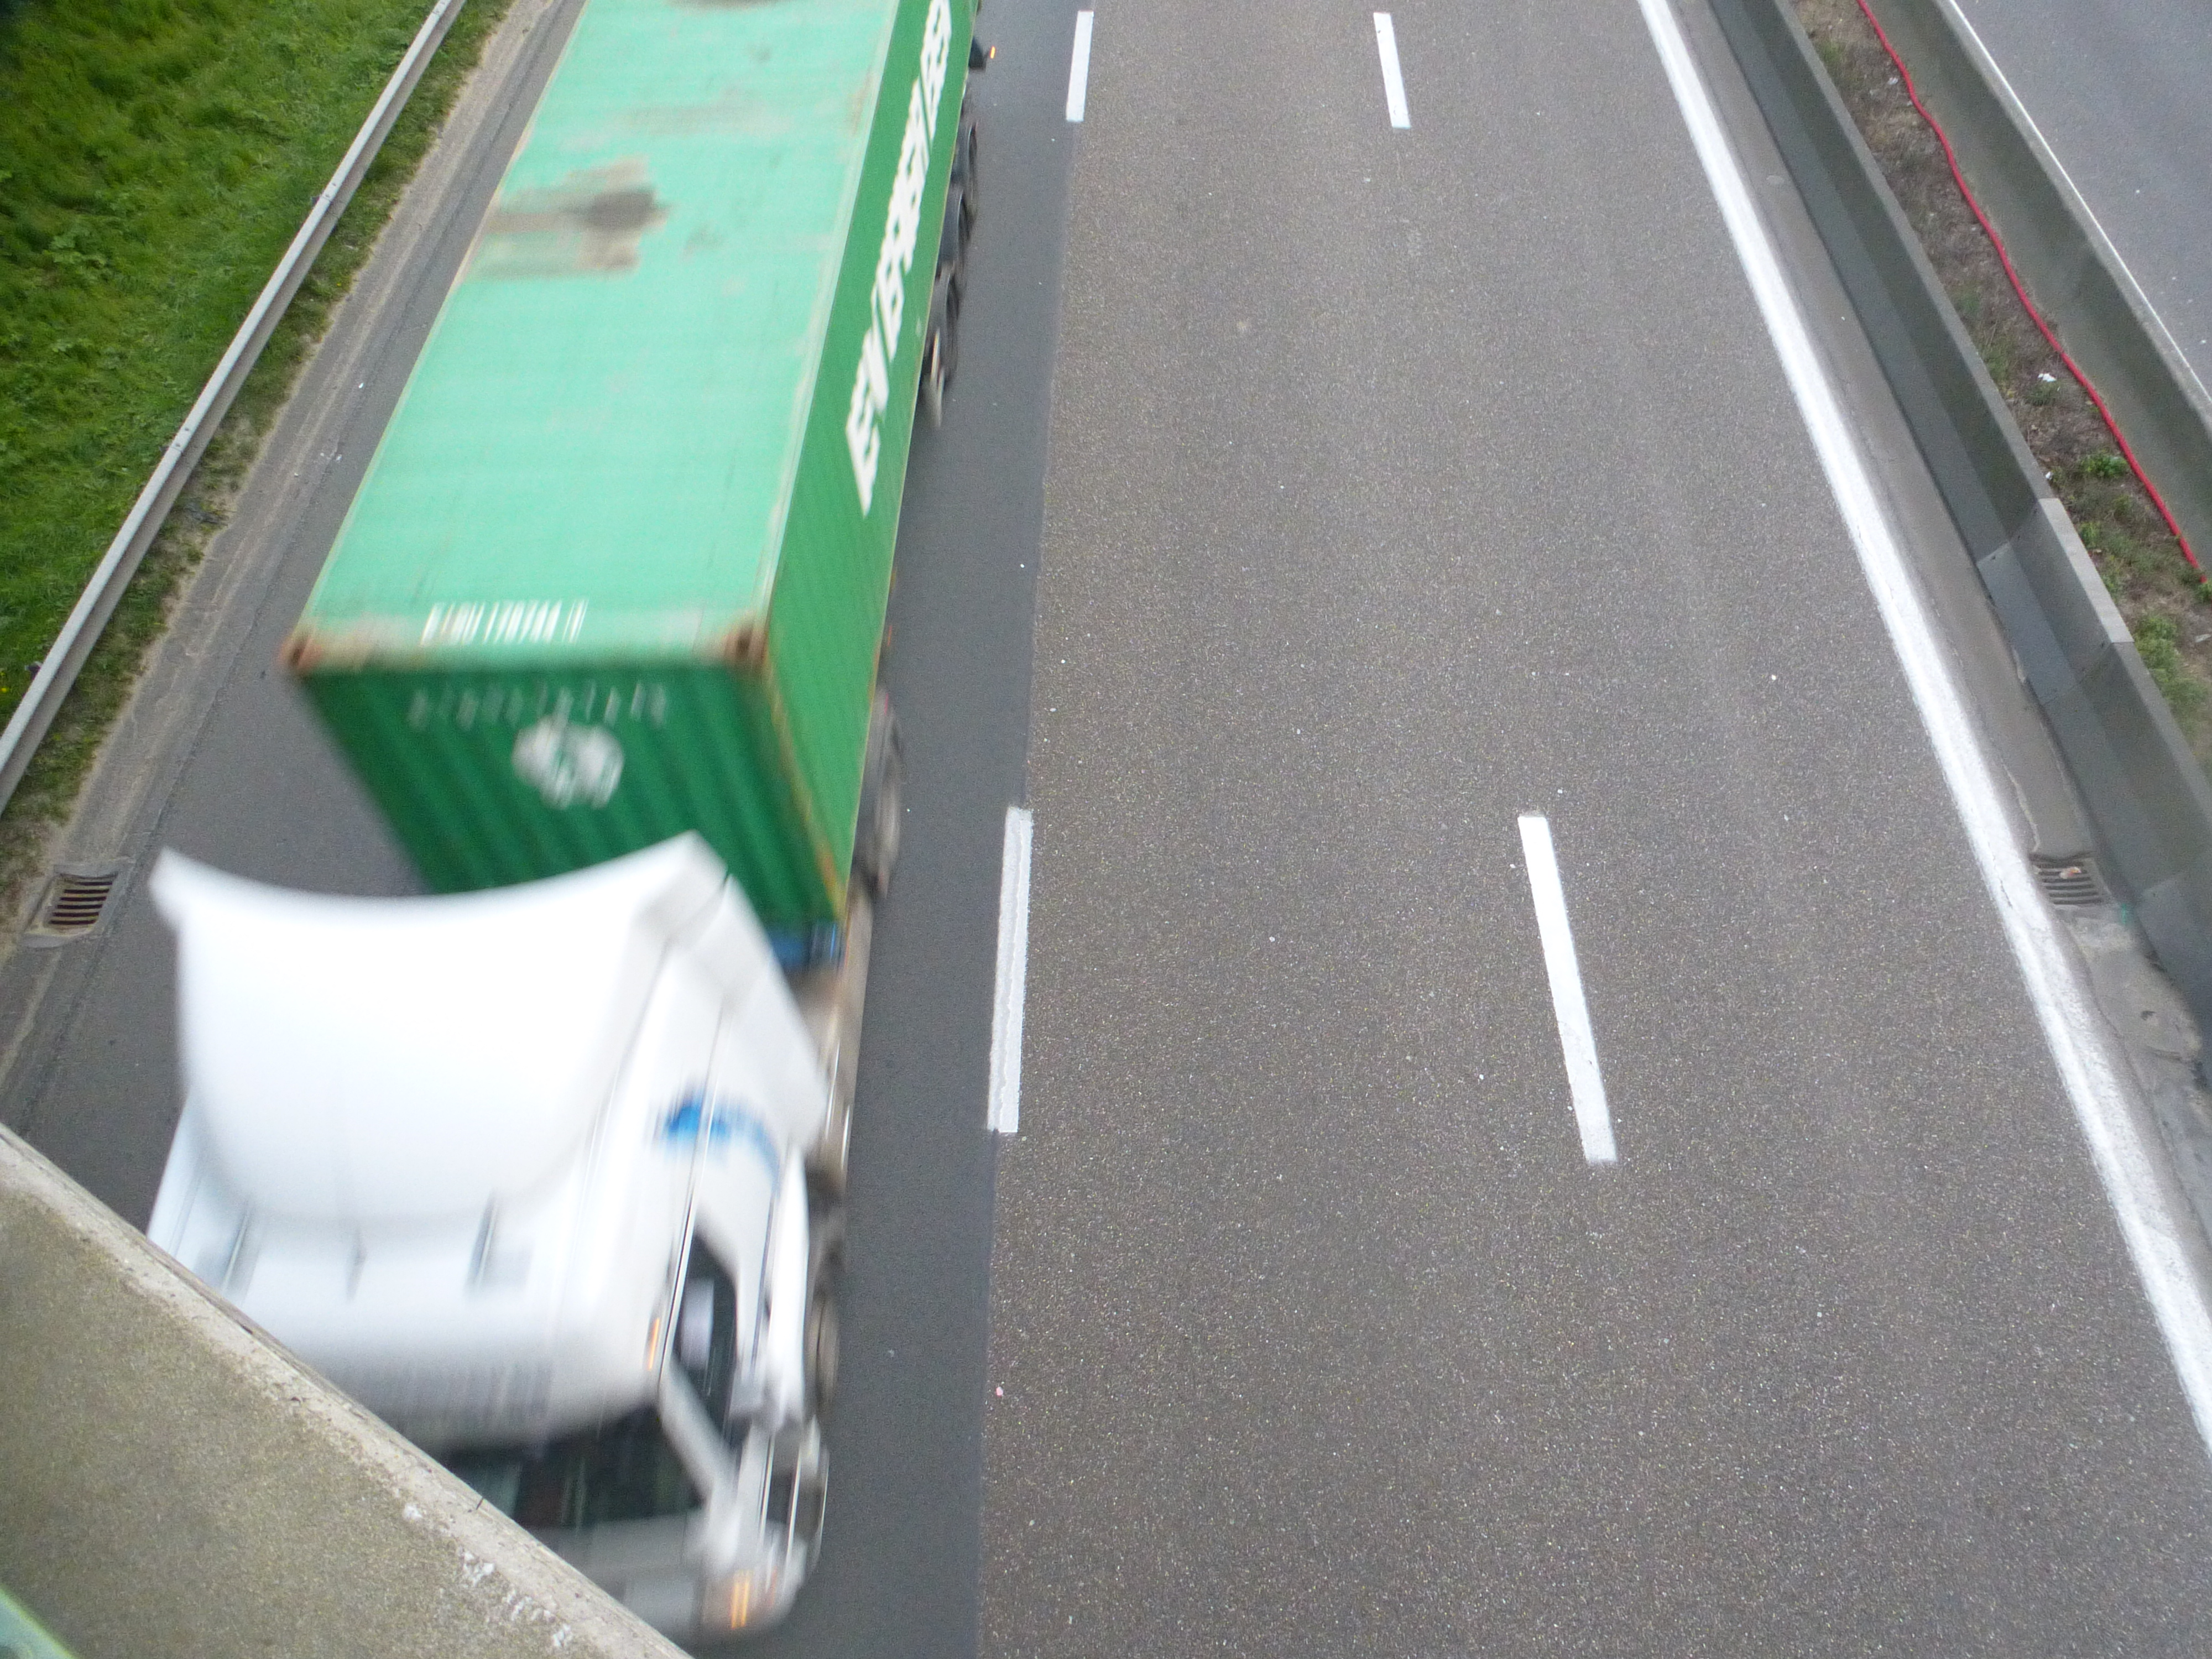
\includegraphics[{width= \textwidth}]{../Images/Camera/Autoroute/fg/16.jpg}
\end{subfigure}
\caption{Images taken by camera video}
\label{fig:AllAut}
\end{figure}

\begin{figure}[h]
\centering
\includegraphics[{width=0.4 \textwidth}]{../Images/Camera/Autoroute/BGDetect/BGDetect.png}
\caption{Background estimation}
\label{fig:AutBG} 
\end{figure} 

\end{frame}

\begin{frame}
	\frametitle{Update of the background}
\begin{enumerate}
	\item Formula
      $$B_{new} = a B_{init} + (1-a) I$$
	Typically, $a = 0.99$
	\item Examples with $a = 0.5$
\end{enumerate}
%	
\begin{figure}[h]
\centering
\begin{subfigure}{0.20\textwidth}
\includegraphics[width= \textwidth]{../Images/Camera/Autoroute/fg/a50/CamDeblurred-1.png}
\end{subfigure}
~
\begin{subfigure}{0.20\textwidth}
\includegraphics[{width= \textwidth}]{../Images/Camera/Autoroute/fg/a50/CamDeblurred-2.png}
\end{subfigure}
~
\begin{subfigure}{0.20\textwidth}
\includegraphics[{width= \textwidth}]{../Images/Camera/Autoroute/fg/a50/CamDeblurred-3.png}
\end{subfigure}
~
\begin{subfigure}{0.20\textwidth}
\includegraphics[{width= \textwidth}]{../Images/Camera/Autoroute/fg/a50/CamDeblurred-4.png}
\end{subfigure}
~
\begin{subfigure}{0.20\textwidth}
\includegraphics[{width= \textwidth}]{../Images/Camera/Autoroute/fg/a50/CamDeblurred-5.png}
\end{subfigure}
~
\begin{subfigure}{0.20\textwidth}
\includegraphics[{width= \textwidth}]{../Images/Camera/Autoroute/fg/a50/CamDeblurred-6.png}
\end{subfigure}
~
\begin{subfigure}{0.20\textwidth}
\includegraphics[{width= \textwidth}]{../Images/Camera/Autoroute/fg/a50/CamDeblurred-7.png}
\end{subfigure}
~
\begin{subfigure}{0.20\textwidth}
\includegraphics[{width= \textwidth}]{../Images/Camera/Autoroute/fg/a50/CamDeblurred-8.png}
\end{subfigure}
~
\begin{subfigure}{0.20\textwidth}
\includegraphics[{width= \textwidth}]{../Images/Camera/Autoroute/fg/a50/CamDeblurred-9.png}
\end{subfigure}
~
\begin{subfigure}{0.20\textwidth}
\includegraphics[{width= \textwidth}]{../Images/Camera/Autoroute/fg/a50/CamDeblurred-10.png}
\end{subfigure}
~
\begin{subfigure}{0.20\textwidth}
\includegraphics[{width= \textwidth}]{../Images/Camera/Autoroute/fg/a50/CamDeblurred-11.png}
\end{subfigure}
\caption{Update of the Background with $a=0.5$}
\label{fig:Udpade}
\end{figure}
\end{frame}

\subsection{Foreground estimation}
\begin{frame}
  \frametitle{Foreground estimation}
  \todo[inline]{Arnaud}
\end{frame}

\subsection{Deconvolution}
\begin{frame}
  \frametitle{Simple adaptations}
  \begin{block}{PSF estimation}
    We need
    \begin{itemize}
      \item Pure blurred image;
      \item Not too small.
    \end{itemize}
    The biggest square of foreground seems good but not necessarily
    pure since it is an upper bound.

    Let's take the biggest square $-3$ pixels at each borders.
  \end{block}
  \begin{block}{Wiener}
    Deblur the subimage then only change pixels of the connected
    shape.
  \end{block}
\end{frame}

\begin{frame}
  \frametitle{``select-lucy''}
  \begin{block}{``select-lucy''}
    Since it is iterative, we can do better than Wiener.
    At \emph{each} iteration, only change pixels of the connected
    shape.
  \end{block}
  \begin{myfig}{select-lucy-zooms}{Zoom on ``select-lucy'' solution.}
    \includegraphics[height=5cm]{dontpanic-40-0_2_1-100_zoom.jpg}
  \end{myfig}
\end{frame}

\begin{frame}[allowframebreaks]
  \frametitle{``exact-lucy''}
  \myfullfig{car-middlediff}{Plot of the diff (foreground $-$ background normalized by variance)}{0.5}
  \begin{block}{``exact-lucy''}
    Absolute value of the slope of the linear regression of $L$ consecutive diffs
    maximized at start and end of background.

    \begin{enumerate}
      \item Estimate the ``exact'' foreground.
      \item Blur it and get an estimate of the ratio of background
        for each pixel.
      \item Remove the background.
      \item Use our modified iteration not sensible to black.
    \end{enumerate}
  \end{block}
  \begin{myfig}{exact-lucy-zooms}{Zoom on ``exact-lucy'' solution.}
    \includegraphics[height=5cm]{dontpanic-40_0-2_2-100_zoom.jpg}
  \end{myfig}
  \begin{block}{Conclusion}
    Lucy-Richardson likes degrees of freedom (recall ``magic-lucy'' success).
  \end{block}
\end{frame}

\subsection{Comparison of results}
\subsubsection{Quality of deblurring}
\begin{frame}[allowframebreaks]{Comparison of results - Sensitivity to noise}

\begin{figure}
\centering
\includegraphics[{scale=0.1}]{../Images/Results/desert/Speckle/input.png}
\caption{Original image whith Speckle noise}
\end{figure}


\begin{figure}
\centering
\begin{subfigure}{0.3\textwidth}
\includegraphics[{width= \textwidth}]{../Images/Results/desert/Speckle/L.png}
\caption{Lucy}
\label{fig:SpeckleL}
\end{subfigure}
~
\begin{subfigure}{0.3\textwidth}
\includegraphics[{width= \textwidth}]{../Images/Results/desert/Speckle/W.png}
\caption{Wiener}
\label{fig:SpeckleW}
\end{subfigure}
~
\begin{subfigure}{0.3\textwidth}
\includegraphics[{width= \textwidth}]{../Images/Results/desert/Speckle/R.png}
\caption{Reguralization}
\label{fig:SpeckleR}
\end{subfigure}
\caption{Image with speckel noise deblurred.}
\end{figure}

\end{frame}


\begin{frame}[allowframebreaks]{Comparison of results - Sensitivity to approximate angle}

\begin{figure}
\centering
\includegraphics[scale = 0.2]{../Images/Results/NimeAngle/Blurlength30angle10.png}
\caption{Artificial blur: $30$ pixels and $10$ degrees}
\label{fig:nimeOriginal}
\end{figure}

\begin{figure}
\centering
\begin{subfigure}{0.3\textwidth}
\includegraphics[width= \textwidth]{../Images/Results/NimeAngle/LucyAngle8.png}
\caption{Lucy}
\label{fig:L8}
\end{subfigure}
~
\begin{subfigure}{0.3\textwidth}
\includegraphics[{width= \textwidth}]{../Images/Results/NimeAngle/WienerAngle8.png}
\caption{Wiener}
\label{fig:W8}
\end{subfigure}
~
\begin{subfigure}{0.3\textwidth}
\includegraphics[{width= \textwidth}]{../Images/Results/NimeAngle/RegAngle8.png}
\caption{Reguralization}
\label{fig:R8}
\end{subfigure}
\caption{Image deblurred with an angle of 8 degrees and the right length.}
\end{figure}

\end{frame}


\begin{frame}[allowframebreaks]{Comparison of results - Sensitivity to approximate length}

\begin{figure}
\centering
\includegraphics[{scale=0.2}]{../Images/Results/Lena/Blur20deg30length/ArtificialBlurred.png}
\caption{Artificial blur: $30$ pixels and $0$ degrees}
\end{figure}

\begin{figure}
\centering
\begin{subfigure}{0.3\textwidth}
\includegraphics[{width= \textwidth}]{../Images/Results/Lena/Blur20deg30length/L40.png}
\caption{Lucy}
\label{fig:L40}
\end{subfigure}
~
\begin{subfigure}{0.3\textwidth}
\includegraphics[{width= \textwidth}]{../Images/Results/Lena/Blur20deg30length/W40.png}
\caption{Wiener}
\label{fig:W40}
\end{subfigure}
~
\begin{subfigure}{0.3\textwidth}
\includegraphics[{width= \textwidth}]{../Images/Results/Lena/Blur20deg30length/R40.png}
\caption{Reguralization}
\label{fig:R40}
\end{subfigure}
\caption{Image deblurred with length estimation = $40$ pixels and correct angle.}
\end{figure}

\end{frame}

\subsubsection{Computation time}
\begin{frame}{Comparison of results - Computation time}
\begin{figure}[h!]
\centering
\begin{subfigure}{0.4\textwidth}
\includegraphics[{width= \textwidth}]{../Images/ComplexityRel.png}
%\caption{time needed to compute `` the picture/ the smallest picture'' - y-axis and number of pixels of the `` picture / smallest picture'' - x-axis.}
\end{subfigure}~
\begin{subfigure}{0.4\textwidth}
\includegraphics[{width= \textwidth}]{../Images/ComplexityAbs.png}
%\caption{Time  needed to compute the picture on the y-axis, number of pixels of the picture on the x-axis.}
\end{subfigure}
\caption{Complexity of our different algorithms. The blue line is for \texttt{deconvLucy} (16 iterations), the red one for \texttt{deconvwnr} and the green one for \texttt{deconvreg}.}
\label{fig:Complexity}
\end{figure}

\end{frame}
\subsubsection{Conclusion}
\begin{frame}{Comparison of results - Conclusion}
\begin{itemize}
\item Lucy : the most robust but the slowest when the number of pixels rises 
\begin{itemize}
\item if low number of pixels or some time available;
\end{itemize}
\item Wiener : the fastest but some times poor results 
\begin{itemize}
\item Good compromise;
\end{itemize} 
\item Regularisation : the most sensitive to errors 
\begin{itemize}
\item sould be avoided, slower and worse than Wiener.
\end{itemize}
\end{itemize}

\end{frame}


\section[Future Develop.]{Future Development}
%\section[Conclus.]{Conclusion}
\section[Ccl.]{Conclusion}
\begin{frame}
\frametitle{ Thanks for your attention}
\begin{center}
\textbf{ Any questions ? }
\end{center}
\end{frame}

\end{document}
